\documentclass[12pt]{jsbook}
\usepackage{style/pethesis}
\usepackage{amsmath,amssymb,bm}
\usepackage{caption}
\usepackage{minitoc}
\usepackage{hhline}
%\usepackage{style/algorithmic}
%\usepackage{style/algorithm}
\usepackage{algorithmic}
\usepackage{algorithm}
\usepackage{booktabs}
\usepackage[dvipdfmx]{graphicx} 
%\usepackage[dvipdfmx,draft]{graphicx} %画像を表示せず枠だけ確保しコンパイル時間減らす
\usepackage[dvipdfmx, usenames]{color}
\usepackage{colortbl}
\usepackage{ascmac}
\usepackage{lscape}
\usepackage{url}
\usepackage{graphicx}
\usepackage{float}
\usepackage{siunitx}
\usepackage{comment}
\usepackage{enumerate}

% 丸付き文字
\newcommand{\maru}[1]{{\ooalign{\hfil
 \ifnum#1>999 \resizebox{.25\width}{\height}{#1}\else%
 \ifnum#1>99 \resizebox{.33\width}{\height}{#1}\else%
 \ifnum#1>9 \resizebox{.5\width}{\height}{#1}\else #1%
 \fi\fi\fi%
\/\hfil\crcr%
\raise.167ex\hbox{\mathhexbox20D}}}}

%\renewcommand{\figurename}{Fig. }
%\renewcommand{\tablename}{Table }
\newcommand{\argmax}{\mathop{\rm arg~max}\limits}
\newcommand{\argmin}{\mathop{\rm arg~min}\limits}
\usepackage{threeparttable}

\usepackage[subrefformat=parens]{subcaption}
\captionsetup{compatibility=false}
%\usepackage{otf}

% ++++++++++++++++++++++++++++++++++++++++++++++++++++++++++++++++ %
%   論文の表紙の項目
% ++++++++++++++++++++++++++++++++++++++++++++++++++++++++++++++++ %
\thesistype{令和2年度 卒業論文}
\title{タイコグラフィ法による \vspace{2mm} \\ 大型X線ウォルターミラーの光学的評価}
\etitle{Wave-optical evaluation of large-scale Wolter X-ray mirrors \vspace{2mm} \\ by ptychography measurement}
\affiliation{東京大学 工学部 精密工学科}
\supervisor{三村 秀和 准教授}
\studentid{03-190395}
\author{{\LARGE 渡辺貴史}}
\begin{document}
\dominitoc
%title
\maketitle

%abstract
%\thispagestyle{empty}
%\chapter*{概要}
\markboth{概要}{}
\label{abst}
\def\thepage{}
\thispagestyle{empty}

あああ\vspace{12pt}

いいい\vspace{12pt}

ううう\vspace{12pt}

えええ
\thispagestyle{empty}

\newpage
%%%%%%%%%%%%%%%%%%%%%%%%%%%%%%%%%%%%%%%%%%%%%%%%%%%%%%%%%%%%%%%%%%%%%%%%%%%%%%%

%%%%%%%%%%%%%%%%%%%%%%%%%%%%%%%%%%%%%%%%%%%%%%%%%%%%%%%%%%%%%%%%%%%%%%%%%%%%%%%
%%% Local Variables:
%%% mode: katex
%%% TeX-master: "../thesis"
%%% End:


\frontmatter
%table of contents
\tableofcontents
%table of figures
\listoffigures
%table of tables
\listoftables

% ++++++++++++++++++++++++++++++++++++++++++++++++++++++++++++++++ %
%   Main Body
% ++++++++++++++++++++++++++++++++++++++++++++++++++++++++++++++++ %
\mainmatter
\chapter{序論}
\thispagestyle{empty}
\label{chap1}
\graphicspath{{chap1/figure/}}
\minitoc

%%%%%%%%%%%%%%%%%%%%%%%%%%%%%%%%%%%%%%%%%%%%%%%%%%%%%%%%%%%%%%%%%%%%%%%%%%%%

% ================================================== %
% section
% ================================================== %
\newpage
\section{X線天文分野におけるミラー結像系}
\label{chap1_imaging_mirror_in_astronomy}
太陽の活動を理解することは、天文分野において重要な意味を持ち、未だに残る多くの謎に対して現在も多くの努力がなされている。
中でも、太陽の中心核から光球に向かって6000℃まで温度が下がっていくのに対し、そこからはるか上空にあるコロナが100万℃の高温状態であることは「コロナ加熱問題」として知られ、他の銀河系における高温プラズマの発生原理を解明する上でも非常に重要な問題として位置づけられている。\cite{ShimizuToshifumi2018}
非常に高温な現象であるため、それはX線領域の電磁波を検出することによって観測でき、数百eVから1keV以下の軟X線領域と数keVから数十keVの硬X線領域の観測によってそれぞれ得られる情報がある。
このようなX線領域の天体観測においては、効率と受光面積の観点から基本的にミラーによる結像系が用いられる。
X線は大気によって吸収されやすいため、太陽コロナのX線領域での観察は大気圏外に打ち上げられた宇宙船上で行われるのが望ましく、飛行中の振動に耐えうる系が構成されなければならない。
また、コロナ加熱問題などの現象解明のためには、経時的な変化を追う必要があるため、観測中の結像系の安定が求められる。

\clearpage
% -------------------------------------------------- %
% section
% -------------------------------------------------- %
\newpage

\section{Wolterミラー}
\label{chap1_wolter_mirror}

この要求に対して非常に有用なのが、2回反射により角度誤差耐性を強めたWolterミラーである。\cite{1952AnP...445...94W}

十分遠方にある天体を観測する際、それが発するまたは反射する光はほぼ平行光とみなせる。
放物線の持つ平行線を反射して焦点に集めるという効果を利用して、放物線を軸回りに回転した曲面で平行光を反射し1点に集める光学素子が回転放物面ミラーである。
全周に渡って回転した回転放物面ミラーは、円形に広がる平行光に対してこれを1点に集光する。

しかし、回転放物面には設置角度の誤差に弱いという欠点が存在する。
これを解決するのが、2回反射型のミラーである。
図\ref{fig:wolter_robustness}に示すように、2つの面が固定されているようなミラーについて1回ずつ反射をすると、最終的に出射される光の進行角度は設置角度誤差の影響を受けない。

\begin{figure}[b]
\centering
\includegraphics[width=10cm]{wolter_robustness.png}
\caption{2回反射による設置角度誤差のキャンセル}
\label{fig:wolter_robustness}
\end{figure}

このことは、2回反射が設置角度誤差に対して安定した結像性能を持つことの大きな理由である。
また、Wolter I型ミラーは近似的にアッベの正弦条件を満たす。
無限遠の光源に対するアッベの正弦条件は図\ref{fig:abbe_sine_condition_for_parallel_light}の変数について
\[
    h = f \sin u
\]
と表される。


\begin{figure}[b]
\centering
\includegraphics[width=10cm]{wolter_type_3.png}
\caption{無限遠の光源に対するアッベの正弦条件}
\label{fig:abbe_sine_condition_for_parallel_light}
\end{figure}

アッベの正弦条件を満たすとき、光軸に対して角度がついた平行光に対して球面収差とコマ収差のない結像系であると言える。

2回反射を利用した集光ミラーであって、全周にわたって回転したものをWolterミラーという。
2回の反射面は、放物線、双曲線、楕円の3種類の2次曲線を組み合わせた図形の回転体として与えられる。
焦点を共有するように設計・配置することで1点に集光する系を構成することができる。
WolterミラーにはI型(図\ref{fig:wolter_type_1})、II型(図\ref{fig:wolter_type_2})、III型(図\ref{fig:wolter_type_3})の3種類が存在する。
I型は放物面、双曲面の順に反射する。
いずれも内面で反射する形状になっているため、\ref{chap1_wolter_fabrication_process}節で述べるマンドレル転写加工がしやすく高精度な作製が期待できる。
また、受光面積を広げるため、\ref{chap1_nested_wolter_mirror}節で述べるような複数枚のネスト構造を構成することが比較的容易である。
II型は放物面内面、双曲面外面の順に反射する構成になっている。
I型に比べ加工・設置が難しくなるが、2枚が覆いかぶさるように重ねた配置にすることができ、焦点距離を短くし光学系全体を小型化することができる。
III型も同様に加工・設置が難しくなるが、焦点距離を短くするような配置が可能になる。
II型、III型は凸面形状ミラーの加工の困難さからWolterミラーとしては実用化されていない。
KB型配置ではIII型に対応する構成での集光光学系が提案されている。\cite{Yamada:20}

\begin{figure}[b]
\centering
\includegraphics[width=10cm]{wolter_type_1.png}
\caption{Wolter I型}
\label{fig:wolter_type_1}
\end{figure}

\begin{figure}[b]
\centering
\includegraphics[width=10cm]{wolter_type_2.png}
\caption{Wolter II型}
\label{fig:wolter_type_2}
\end{figure}

\begin{figure}[b]
\centering
\includegraphics[width=10cm]{wolter_type_3.png}
\caption{Wolter III型}
\label{fig:wolter_type_3}
\end{figure}

\subsection{ネスト型Wolterミラー}
\label{chap1_nested_wolter_mirror}

Wolterミラーのような円筒形のミラー、特にX線を反射するため斜入射角が小さく設計されたミラーにおいて、中空になっている内側部分を通過する光を集めることができず、集光強度を高める上で不都合である。
これを解決する方法として、図\ref{fig:nested_wolter_mirror}のように口径の異なるWolterミラーを内側に挿入するというものがある。\cite{BuitragoCasas2017}

\begin{figure}[b]
\centering
\includegraphics[width=8cm]{nested_wolter_mirror.png}
\caption{Nested Wolterミラーの例}
\label{fig:nested_wolter_mirror}
\end{figure}

このようにネスト構造にすることで、受光面積を大きくすることができ、集光強度を上げることができる。
このようなネスト構造を構成できるのはI型のみであり、その点で天体応用としてはI型が有力な選択肢となる。
実際、FOXSI3でもI型をネストしたNested Wolterミラーが搭載されていた。
このように受光面積の観点では非常に有利であるNested Wolterミラーだが、ネストする枚数を増やすほどその設置が困難になるという問題がある。
ミラー同士の角度・光軸のずれなど、調整しなければならない誤差要因が増えるためである。
そのため、ネストの構成後に光学系を統合的に計測する方法が必要になる。
また、ミラー同士をネストさせたあとにプローブを挿入して計測することは困難であるため、その統合的な評価は間接測定によって行われなければならない。

\newpage
\section{FOXSI4におけるWolterミラー}
\label{chap1_background}

\subsection{FOXSI4}
\label{chap1_foxsi}

2018年に打ち上げられたFOXSI3では太陽コロナのX線写真を撮影することに成功した。\cite{weko_20796_1}
図\ref{fig:foxsi-fullsun-image}はその撮影像の1枚である。
FOXSI3よりも高い分解能で太陽コロナの像を撮影することを目標として、光学系をアップデートしたFOXSI4が2023年頃の打ち上げを予定している。\cite{2019AGUFMSH31C3315V}
ここで搭載されるWolterミラーについて、作製精度を

\begin{figure}[h]
\centering
\includegraphics[width=6cm]{foxsi3-full-sun.png}
\caption{FOXSI-3 phoenix full sun soft X-ray image \cite{weko_20796_1}}
\label{fig:foxsi-fullsun-image}
\end{figure}

\subsection{Wolterミラーの設計}
\label{chap1_wolter_arrangement}
FOXSI4に搭載予定のX線用Wolterミラーは、放物面、双曲面の順に反射するI型に分類される。

以下では、開発対象となっているWolter I型のミラーの設計パラメータを図\ref{fig:wolter_params}に対応して表\ref{tb:wolter_params}に示す。

\begin{figure}[h!]
\centering
\includegraphics[width=12cm]{wolter_mirror_params.png}
\caption{Wolterミラーの設計変数}
\label{fig:wolter_params}
\end{figure}

\begin{table}[ht]
\begin{center}
  \begin{tabular}{|c|c|l|} \hline
    変数 & 値 & 説明 \\ \hline
    $d_u$ & 60.801 mm & 上流端開口直径 \\
    $d_s$ & 60.000 mm & 接合部直径 \\
    $d_d$ & 57.689 mm & 下流端開口直径 \\
    $l_p$ & 102.501 mm & 放物面部長さ \\
    $l_h$ & 97.499 mm & 双曲面部長さ \\
    $ml$ & 200.000 mm & ミラー全長 \\
    $f$ & 2000.000 mm & 焦点距離 \\ \hline
  \end{tabular}
  \caption{Wolterミラー各設計変数の値}
  \label{tb:wolter_params}
\end{center}
\end{table}

これらを図\ref{fig:wolter_profile}のように放物面部および双曲面部の設計半径として表すと、下式(パラメータは図\ref{tb:wolter_profile_constants})のようになる。
$f1$は座標系の平行移動に関して任意であるため、変数として表記する。

\begin{equation}
    r_p(z) = \sqrt{ -4p(z - p - f_2) } \\
\end{equation}

\begin{equation}
    r_h(z) = b \sqrt{ \frac{(z - (f_1 + f2) / 2)^2}{a^2} - 1.0 }
\end{equation}

\begin{figure}[h]
\centering
\includegraphics[width=10cm]{mirror_profile.png}
\caption{Wolterミラーの設計半径}
\label{fig:wolter_profile}
\end{figure}

\begin{table}[htb]
    \begin{center}
      \begin{tabular}{|c|c|l|} \hline
        定数 & 値 & 説明 \\ \hline
        $p$ & 0.0562 mm & 下流端開口直径 \\
        $a$ & 1000.056 mm & 放物面部長さ \\
        $b$ & 10.606 mm & 双曲面部長さ \\ 
        $f_1$ & 任意 & 焦点座標 \\
        $f_2$ & $f_1 + 2 \sqrt{ a^2 + b^2 }$  & 共焦点座標 (双曲線のもう一方の焦点) \\\hline
      \end{tabular}
      \caption{Wolterミラーの設計半径における定数}
      \label{tb:wolter_profile_constants}
    \end{center}
\end{table}


\subsection{マンドレル電鋳法}
\label{chap1_mirror_mandrel}

ここで、測定対象となるWolterミラーの製造プロセスについて述べる。
凹状になっている回転体形状のミラー内面を高精度に加工することは難しく、凸形状のマンドレルを高精度に加工し、これに対してさらに転写加工を行うという手法が提案されている。\cite{Mimura2018}
図\ref{fig:mandrel_plating_pictures}に回転楕円ミラーに対するマンドレル電鋳法の一連の流れを示す。

\begin{figure}[!ht]
\centering
\subfloat[高精度に加工されたマンドレル]{
    \includegraphics[width=4cm]{mandrel_before_plating.png}
    \label{fig:mandrel_before_plating}
}
\subfloat[マンドレルに転写されたミラー]{
    \centering
    \includegraphics[width=4cm]{mandrel_after_plating.png}
    \label{fig:mandrel_after_plating}
}
\subfloat[取り外されたミラー]{
    \centering
    \includegraphics[width=4cm]{detached_mirror.png}
    \label{fig:detached_mirror}
}
\caption[]{マンドレル電鋳法の模式図}
\label{fig:mandrel_plating_pictures}
\end{figure}

3種類のWolterミラーのうち、2回の反射が内面において起こるI型では、同様の手法で加工が可能であり、既にこの方法で真円度誤差\SI{20}{\micro \metre}程度以下の精度でWolterミラーが作製されている。\cite{Egawa2019}

\subsection{直接計測法}
\label{chap1_direct_measurement}

久米らは、図\ref{fig:profile_measurement_schematic}および図\ref{profile_measurement}に示すように、接触式変位計を用いて周方向形状誤差プロファイルおよび長手方向形状誤差プロファイルを数本ずつ取得し、さらにこれらを組み合わせることで3次元形状を決定するという方法を提案した。\cite{Kume2017}
しかしこれらの誤差プロファイル計測手法では、ある始点からの変位量しか測定できず、直径や長手プロファイルの傾き(テーパー角)の情報を取得することができない。
このような誤差プロファイル計測では得られない情報を補完する計測方法が必要である。
また、高精度に加工されたミラー内面に接触式のプロファイル計測を適用することは、その表面形状を悪化させる恐れがある。
そのため、非接触式の計測方法を用いることが望ましい。

\begin{figure}[h]
\centering
\includegraphics[width=5cm]{profile_measurement_schematic.png}
\caption{接触式誤差プロファイル計測}
\label{fig:profile_measurement_schematic}
\end{figure}

\begin{figure}[!ht]
\centering
\subfloat[長手方向形状誤差プロファイル]{
    \centering
    \includegraphics[height=4cm]{meridional_profile.png}
    \label{fig:meridional_profile}
}
\subfloat[周方向形状誤差プロファイル]{
    \centering
    \includegraphics[height=4cm]{sagital_profile.png}
    \label{fig:sagital_profile}
}
\subfloat[3次元形状誤差プロファイル]{
    \centering
    \includegraphics[height=4cm]{combined_profile.png}
    \label{fig:combined_profile}
}
\caption[]{プロファイル計測による3次元プロファイルの構成}
\label{fig:profile_measurement}
\end{figure}



\clearpage
% -------------------------------------------------- %
% section
% -------------------------------------------------- %
\newpage
\section{波面計測法によるミラー形状の解析}
\label{chap1_wave_metrics}

プロファイル計測では得られない情報を取得すること、またネスト構造のミラーを計測可能な間接測定であることという2つの要請を満足させる方法として、波動光学の理論を応用した波面計測法がある。
波動光学では、光波を複素スカラー場$U(P)=A(P)\exp(i\Phi(P))$とし、等位相面$\Phi(P)=const$を波面とよぶ。
一般に、ある光が1点に収束するとき、光の波面は収束点を中心とする球面になる。
もし仮にミラーが入射光を完全に1点に集めるとすると、ミラーの出口、下流端開口に現れる光波は球面波になるはずだが、現実にはミラーの設計の特徴や加工時の誤差を反映して波面が変形する。
波面計測法とは、この波面のずれを波面誤差$\Delta\Phi(P)/k$(長さの次元を持つ)として求め、波面誤差からその原因となる誤差の量を算出するという計測方法である。
可視光光源に対する波面の計測手法として広く利用されているのが、シャックハルトマンセンサーである。
シャックハルトマンセンサーすごいよね
しかし、非常に細い輪帯とシャックハルトマンセンサーは相性が悪く


\clearpage
% -------------------------------------------------- %
% section
% -------------------------------------------------- %
\newpage

\section{本研究で測定対象となるWolterミラー}
\label{chap1_target_wolter}

\subsection{天文用X線Wolterミラーの持つ特性}
\label{chap1_wolter_specific_feature}

口径が大きく、X線に対応するため射入射角を小さく設定したWolterミラーはNAがやや小さくなり、波面計測において求めなければならない波面は図\ref{fig:wolter_thinring}に示すように非常に細い輪帯状になる。
輪帯の幅(外円と内円の半径の差)は実に\SI{363.3}{\micro \metre}であり、波面計測に求められる空間分解能は非常に高いものとなる。
半径方向の位相分布を見る際、極値を取っている状態を判別するには、少なくとも3ピクセルに分割できている必要があり、\SI{100}{\micro \metre}程度の空間分解能で計測できなければならない。
波面精度を十分に確保しつつ、空間分解能が十分に高い波面計測法を開発する必要がある。

\begin{figure}[h!]
\centering
\includegraphics[width=7cm]{wolter_thinring.png}
\caption{Wolterミラー下流端面における集光波面}
\label{fig:wolter_thinring}
\end{figure}


\clearpage
% -------------------------------------------------- %
% section
% -------------------------------------------------- %
\newpage
\section{本論文の目的}
\label{chap1_purpose}

JAXAの進めるミッションLynxでは、0.5秒角分解能の望遠鏡の搭載を大きな目標として掲げている。\cite{Gaskin2019}
これに先立って、2023年に打ち上げられるFOXSI4に搭載するWolterミラーの加工について、1秒角分解能を目標として設定する。
これを実現する上で問題となる加工誤差はどのようなものであるかを統合的な計測から測定し、加工プロセスへ直ちにフィードバックするための系を開発することが、本研究の目的となる。

% -------------------------------------------------- %
% section
% -------------------------------------------------- %
\section{本論文の構成}
\label{chap1_outline}

\ref{chap2}章では、測定対象のWolterミラーに対して様々な種類の誤差を与え、その際の集光波面の変化をシミュレーションする。
この集光波面の強度分布から、目標とする1秒角分解能の達成に際して要求される許容誤差の範囲を見積もるとともに、\ref{chap3}章以降で扱う波面計測法における解析に用いる基底を前もって解析しておく。
\ref{chap3}章では、波面計測における様々な手法の中でWolterミラーの計測に適した方法を検討するため、シミュレーションによってその利点・欠点を洗い出し、最終的に計測に用いる方法を決定する。
\ref{chap4}章では、\ref{chap3}章で提案された手法について、ミラーに比べ加工誤差が小さく、より理想的な集光が期待できるレンズを用いて、その正当性を実証する。
\ref{chap5}章では、実際に加工された3枚の天文用Wolterミラーに対して計測実験を行い、\ref{chap2}でシミュレーションによって求めた誤差応答との比較からミラー内部形状の誤差に関する解析を行う。
最後に、\ref{chap6}章で考察、結論および今後の展望について述べる。

%%%%%%%%%%%%%%%%%%%%%%%%%%%%%%%%%%%%%%%%%%%%%%%%%%%%%%%%%%%%%%%%%%%%%%%%%%%%%
%%% Local Variables:
%%% mode: katex
%%% TeX-master: "../thesis"
%%% End:

\chapter{Wolterミラーの誤差応答シミュレーション}
\thispagestyle{empty}
\label{chap2}
\graphicspath{{chap2/figure/}}
\minitoc

\newpage
%%%%%%%%%%%%%%%%%%%%%%%%%%%%%%%%%%%%%%%%%%%%%%%%%%%%%%%%%%%%%%%%%%%%%%%%%%%%%


% ================================================== %
% section
% ================================================== %
\section{諸言}
\label{chap2_introduction}

Wolterミラーを光学系に組み込んで利用する際、大きく分けて2つの誤差によってその理想の集光・結像が損なわれる。
ひとつは設計曲面と実際に加工されたミラー表面の形状の誤差、もうひとつはミラー設置時の位置・姿勢の誤差である。
誤差応答、すなわちこれらの誤差が存在する際に集光点の様子がどのように変化するかを調べることで、Wolterミラーの利用時に求められる性能を発揮する上で許容される誤差の量が計算できる。
また、可視光光源を用いた位相回復法によってこれらの許容誤差範囲に収まっているかどうか判定することが可能であるかどうかを知る必要がある。
これらを踏まえ、本章では3段階に渡って誤差応答シミュレーションを行う。
まず、実際にWolterミラーが用いられるX線領域のうち2つの代表的な波長について、各種の誤差を入力した際の集光波面を算出し、許容できる誤差量を計算する。
続いて、ちょうど許容誤差の限界値ぶんの誤差がミラーに存在する場合に可視光を入射した際の位相分布を計算し、可視光による測定が可能であるかどうか、また可能であるならばどういった測定仕様を満たす必要があるかを計算する。
最後に、可視光計測において位相回復法から得られる波面誤差分布から各種誤差への分解を行うため、それぞれの誤差に対応する波面誤差分布をZernike多項式によって表現する。

\clearpage
% ================================================== %
% section
% ================================================== %
\newpage
\section{誤差の評価と許容される誤差}
\label{chap2_beam_evaluation_standard}

理想の集光波面との差異を定量的に評価するためには、具体的な評価軸が必要である。
そこで主に用いられるのが、Strehl比、HPD、FWHMの3つの特徴量である。

\subsection{Strehl比}
\label{chap2_strehl_ratio}
主に集光光学系の文脈において、理想の集光状態を「回折限界集光」と呼ぶ。
回折限界集光の状態にあるかどうかを判別する1つの指標として用いられるのが、Strehl比である。
Strehl比とは、実際の集光波面における最大値と回折限界時の集光波面における最大値の比として定義される。
つまり、振幅を$I(\mathbf{r})$として

\[
r_{\mathrm{Strehl}} = \frac{ \max{\sqrt{I(\mathbf{r})} } }{ \max{ \sqrt{I_{\mathrm{ideal}}( \mathbf{r} )} } }
\]

と定まる。
図\ref{fig:strehl_explanation}にその模式的なグラフを示す。
Strehl比を評価する基準として、Marechal基準\cite{BornWolf:1999:Book}が知られている。
Marechal基準では、Strehl比が0.8以上であるときその系は回折限界集光をしている、とする。
この0.8という値には体系的な根拠はなく、解析・実験における経験的な指標として扱われている。
本論文では、この慣例を踏襲し、0.8を閾値としてStrehl比を評価する。

\begin{figure}[h]
\centering
\includegraphics[width=10cm]{strehl.png}
\caption{Strehl比計算の模式図}
\label{fig:strehl_explanation}
\end{figure}

\subsection{HPD (Half Power Diameter)}
\label{chap2_hpd}

Strehl比による比較検討では「回折限界集光をしているか」に主眼を置いているが、天文用Wolterミラーのように達成すべき角度分解能が決まっている場合では、直接その分解能要求を満たしているかどうかを判定するのが実用的である。
分解能を決定するのは、焦点面におけるビームの集光サイズであり、これは大きく2つの定義によって議論される。
その一つが、Half Power Diameter(HPD)である。HPDの定義は「焦点面上の全強度の50\%の強度を含む円の直径」である。つまり、
\[
    \sum_{d\leq d_{\mathrm{HPD}}} \sqrt{ I(\mathbf{r}) } = \frac{1}{2} \sum \sqrt{ I(\mathbf{r}) }
\]
を満たすような直径$d_{\mathrm{HPD}}$として定義される。
図\ref{fig:hpd_explanation}にその例を示す。
この赤円の内側の強度総和値は、全体の強度総和値の半分になっている。

\begin{figure}[!ht]
\centering
\includegraphics[width=6cm]{HPD.png}
\caption{HPDの例}
\label{fig:hpd_explanation}
\end{figure}

あるHPDを持つようなのふたつの結像点を分離できるような限界の配置が図\ref{fig:hpd_resolution_limit}のときであるとするならば、1秒角分解能という達成目標は図\ref{fig:hpd_arcsecond}が示すようなHPDで言い換えることができる。
つまり、ミラー上流端中心から半径を見込む角度がちょうど1秒角となるようなHPDが達成目標となる。
具体的には、ミラー上流端開口から焦点面までの距離2.1025 mに対してHPDは\SI{10.19}{\micro \metre}と計算される。
HPDを指標とした評価では、これを基準とする。

\begin{figure}[ht]
\centering
\includegraphics[width=6cm]{hpd_resolution_limit.png}
\caption{解像限界の図}
\label{fig:hpd_resolution_limit}
\end{figure}

\begin{figure}[ht]
\centering
\includegraphics[width=12cm]{hpd_arcsecond.png}
\caption{HPDと結像分解能の関係}
\label{fig:hpd_arcsecond}
\end{figure}


\subsection{FWHM (Full Width Half Maximum)}
\label{chap2_fwhm}

HPDに並んでビーム集光サイズの評価として用いられるのが、FWHM(Full Width Half Maximum)である。
こちらは焦点面を集光点を通る直線によって切断したプロファイルに対して、「焦点面における最大値の半分の値を取る2点の距離」と定められる。
図\ref{fig:fwhm_explanation_profile}は1つのプロファイルに対するFWHMの例である。
切断する直線には任意性があるため、通常は図\ref{fig:fwhm_explanation}のように水平方向と鉛直方向の2方向に関して切断しこれを評価する。
\ref{chap2_ideal_focusing}節で具体的な計算例を示すが、結像性能の強いWolterミラーはメインピークに対して比較的大きいサブピークが細かく連なるような集光面強度分布を持つ。
そのため、強度はメインピークより外側に広がって存在しており、解像限界を決める上ではHPDの方が適していると言える。
FWHMはミラー開発の目標に対する評価ではなく、本研究中でのパラメータ設定の指標として用いることとする。

\begin{figure}[ht]
\centering
\includegraphics[width=8cm]{FWHM.png}
\caption{FWHMの例}
\label{fig:fwhm_explanation_profile}
\end{figure}

\begin{figure}[!ht]
\centering

\subfloat[horizontal]{
    \includegraphics[width=5cm]{FWHM_horizontal.png}
    \label{fig:fwhm_explanation_horizontal}
}
\subfloat[vertical]{
    \centering
    \includegraphics[width=5cm]{FWHM_vertical.png}
    \label{fig:fwhm_explanation_vertical}
}
\caption[]{切断の例 水平:\subref{fig:fwhm_explanation_horizontal}, 鉛直:\subref{fig:fwhm_explanation_vertical}}
\label{fig:fwhm_explanation}
\end{figure}


\clearpage
% ================================================== %
% section
% ================================================== %
\newpage

\section{Wolterミラーにおける光学波動場の伝播}
\label{chap2_wolter_diffraction_apporoximation}

シミュレーションおよび位相回復計算を行うにあたり、測定対象のWolterミラーの光学系において適用するべき波動場伝播の近似公式について検討する。
光学波動場の伝播に関しての詳細は付録において解説する。
まず、1章\ref{chap1_wolter_arrangement}節で示したパラメータについて、Fresnel回折近似の成立条件が成り立っているかどうかを確認する。
Fresnel回折近似が成り立つための条件は、近似で切り捨てる微小項が1 radより十分小さいときであり、これは式\ref{eqn:fresnel_approximation_condition}で表される。
ただし$z$は伝搬距離、$\lambda$は波長、$(x, y), (\xi, \eta)$は実空間および逆空間の座標を表す。

\begin{equation}
\label{eqn:fresnel_approximation_condition}
    \frac{\pi}{4\lambda} \max \left\{ (x-\xi)^2 + (y-\eta)^2 \right\}^2 / z^3 \ll 1
\end{equation}

焦点面を3章\ref{chap3_dynamic_range}節に示したCCDカメラのサイズとして取りこれを計算すると、(左辺)の値は1.645 radとなった。
これは十分小さいとは言えず、Fresnel回折近似を満たしているとは言えない。
しかし、Fresnel回折近似を満たしていない場合でも、計算を進めていく上でそれがほとんど影響を及ぼさない場合がある。
位相回復計算においては数万回の伝搬計算を行うため、1回のコストは最小限であることが好ましい。
そこで、厳密計算であるRayleigh-Sommerfeld回折積分とFresnel回折積分近似の集光面強度分布を比較し、実用上の問題が存在するかどうかを検討する。
まず、表\ref{tb:check_approximation_validity_1}に示すような適当な分割で回折積分を実行し、集光波面分布におけるメインピークのFWHMを調べる。

\begin{table}[!ht]
\begin{center}
  \begin{tabular}{|c|c|} \hline
    項目 & 値 \\ \hline
    波長 & 632.8 nm \\
    画素数 & $2048 \times 2048$ \\
    焦点面ピクセルサイズ & \SI{5.0}{\micro \metre} \\ \hline
  \end{tabular}
  \caption{Fresnel回折近似適用可能性の検討1}
  \label{tb:check_approximation_validity_1}
\end{center}
\end{table}

計算の結果、プロファイルは図\ref{fig:fwhm_approximation}のようになった。

\begin{figure}[ht]
\centering
\includegraphics[width=8cm]{../../chap2/figure/fwhm_approximation.png}
\caption{回折積分計算による簡易的な計算で得られた焦点面強度プロファイル}
\label{fig:fwhm_approximation}
\end{figure}

ここから計算されるFWHMは4ピクセル分の\SI{20}{\micro \metre}であった。
これを踏まえ、メインピークを十分な分割数で観察できるよう焦点面ピクセルサイズが\SI{1}{\micro \metre}になるような表\ref{tb:check_approximation_validity_2}のパラメータで回折積分およびFresnel回折近似を用いた場合の集光面強度プロファイルを計算し、比較を行う。

\begin{table}[!ht]
\begin{center}
  \begin{tabular}{|c|c|} \hline
    項目 & 値 \\ \hline
    波長 & 632.8 nm \\
    画素数 & $4096 \times 4096$ \\
    焦点面ピクセルサイズ & \SI{1.0}{\micro \metre} \\ \hline
  \end{tabular}
  \caption{Fresnel回折近似適用可能性の検討2}
  \label{tb:check_approximation_validity_2}
\end{center}
\end{table}

計算の結果、プロファイルは図\ref{fig:diffraction_comparison}のようになった。
また、2つのプロファイルの差分を取って回折積分の最大値で規格化したグラフが図\ref{fig:diffraction_comparison_normalized_diff}である。

\begin{figure}[!ht]
\centering

\subfloat[プロファイルプロット]{
    \includegraphics[width=6cm]{../../chap2/figure/diffraction_comparison_profile.png}
    \label{fig:diffraction_comparison_profile}
}
\subfloat[規格化されたプロファイル誤差]{
    \centering
    \includegraphics[width=6cm]{../../chap2/figure/diffraction_comparison_normalized_diff.png}
    \label{fig:diffraction_comparison_normalized_diff}
}

\caption[]{Rayleigh-Sommerfeld回折積分とFresnel回折積分のプロファイル比較}
\label{fig:diffraction_comparison}
\end{figure}

差分の絶対値の最大値は0.00242程度となった。
これは十分小さく、実際の計測で生じうるノイズと同程度以下であるため、シミュレーションでの検討および位相回復計算を行う上で致命的な問題をもたらさない。
ゆえに、以降の伝搬計算はFresnel回折近似を用いて行う。


\clearpage
% ================================================== %
% section
% ================================================== %
\newpage


\section{シミュレーションの方法}
\label{chap2_simulation_methodology}

この節では、シミュレーションの方法について述べる。
誤差応答シミュレーションは、図\ref{fig:simulation_schematic}に示すように、ミラー反射光が生成する下流端面における集光ビームの位相分布を求め、そこから焦点面に伝播するという流れに沿って行われる。
多数の条件に対して効率よくシミュレーションを行うため、下流端面上の波動場計算は幾何光学に基づいて行い、また下流端面から焦点面への伝播は\ref{chap2_wolter_diffraction_apporoximation}節に述べたようにFresnel回折近似を用いて計算する。
以下に具体的なシミュレーションの手順を示す。

\begin{enumerate}[\expandafter\maru 1]
  \item 放物面および双曲面について、ミラー表面の表現$f(x, y, z)=0$を理想形状の場合と誤差を考慮した場合それぞれについて与える。理想形状のミラーの場合、これは具体的に式\ref{eqn:parabola_surface_func}および式\ref{eqn:parabola_surface_func}のように与えられる。 \\
    \begin{eqnarray}
        f_p(x, y, z) &=& x^2 + y^2 - \left|4p(z-p-f2)\right| = 0 \label{eqn:parabola_surface_func} \\
        f_h(x, y, z) &=& \frac{\left(z - \frac{(f1 + f2)}{2}\right)^2}{a^2} - \frac{x^2 + y^2}{b^2} - 1 = 0 \label{eqn:hyperbola_surface_func}
    \end{eqnarray}
  \item 次に、図\ref{fig:simulation_raytrace}に示すように、ミラー下流端面を$N \times N$の小領域に分割し、ミラー形状から計算される定義域内の各点について幾何光学に基づいて以下のように光路長を計算することで、集光波面を求める。
    \begin{enumerate}[(1)]
      \item 下流端面上の点をPとする。
        誤差のない理想形状のミラーによって2回の反射の後Pに到達するような入射光線を求める。
        具体的には、焦点からPに向かう光線を双曲面、放物面の順に反射すれば、得られた光線が入射光線となる。
        反射の計算について、反射点は光線と\expandafter\maru 1 で与えた$f(x, y, z)=0$との交点として、また反射光の向きは反射の法則から$\mathbf{r} = \mathbf{i} + 2 (-\mathbf{i} \cdot \mathbf{n}) \mathbf{n}$として計算できる。
      \item 求めた入射光線を初期値として光線位置を$x, y$方向に動かして最適化し、誤差を入力したミラーにおける入射光線を求める。
        最適化計算はBroyden法で行う。
        入射光線の位置$(x, y)$を変数、2回反射後の下流端面における目標の点との位置誤差を目標値$\mathbf{E}$として、$\mathbf{E}=\mathbf{0}$を解けばよい。
        入射光線を$(x, y)$を通る$z$軸に平行な直線として与え、2回反射後の下流端面における目標の点との位置誤差を$\mathbf{0}$に近づけるようにこれを動かす。
      \item 求めた入射光線に対してミラー上流端面から下流端面に至るまでの距離$L$を計算し、点$P$での位相を$k L$(波動場を$\exp(i k L)$)として点$P$に関する計算を終了する。
    \end{enumerate}
  \item 次に、\expandafter\maru 2 で求めた下流端面上の各点$P$に対応する光路から、集光面の光軸方向位置の最適化を行う。
    図\ref{fig:simulation_focal_point_optimize}下流端面から集光点に向かう光線の$z=f$上の分布に対し、重心点と各点の距離の2乗和を$E$とする。
    $E$を最小化するように$f$を変化させることで、収束した$f$と重心点を$G(x_G, y_G)$から焦点位置が$F(x_G, y_G, f)$と定まる。
    初期値には理想の焦点距離$f_1$を与え、最適化は黄金探索によって行う。
  \item 最後に、下流端面から焦点面$z=f$に向かって$(x, y)=(x_G, y_G)$を光軸としてFresnel近似を利用した伝播計算を行う。
\end{enumerate}

\begin{figure}[h]
\centering
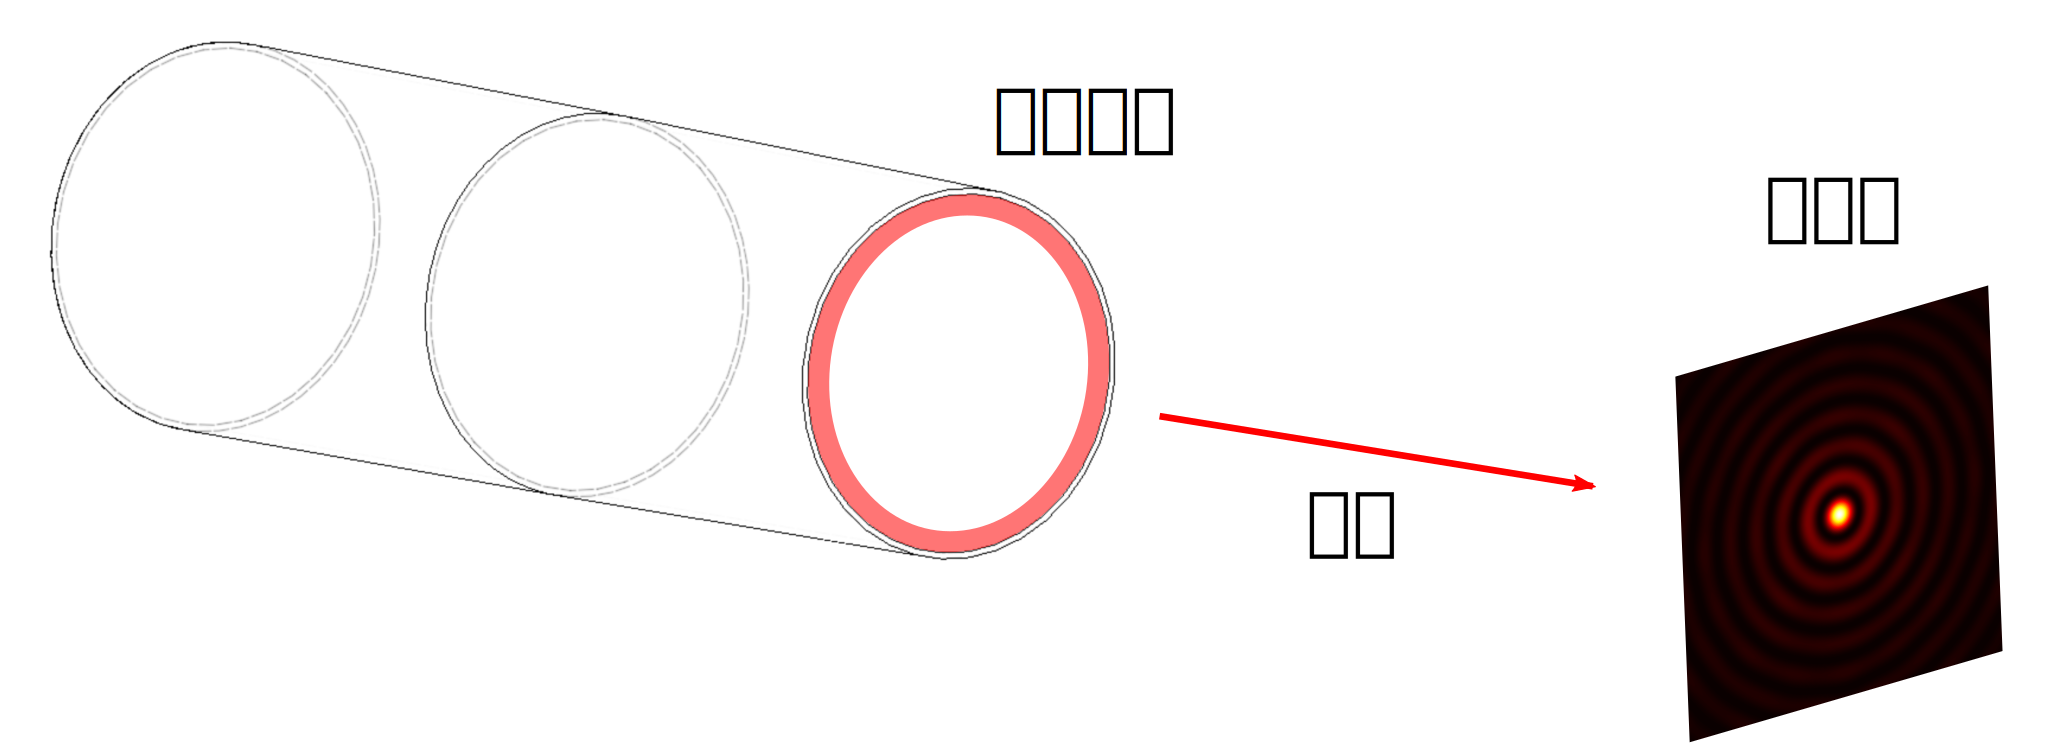
\includegraphics[width=12cm]{method/simulation_schematic.png}
\caption{シミュレーションの概観}
\label{fig:simulation_schematic}
\end{figure}


\begin{figure}[h]
\centering
\includegraphics[width=10cm]{method/simulation_raytrace_schematic.png}
\caption{光線追跡による下流端面波動場の計算}
\label{fig:simulation_raytrace}
\end{figure}

\begin{figure}[h]
\centering
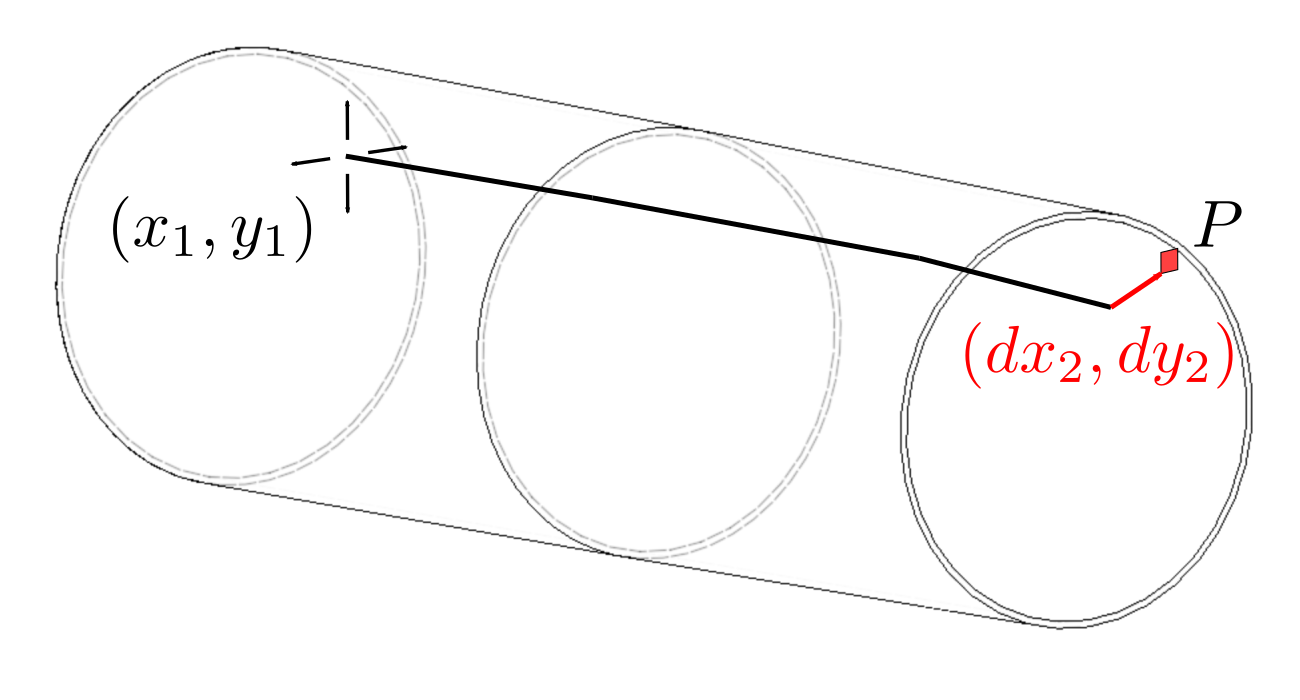
\includegraphics[width=10cm]{method/simulation_backtrace.png}
\caption{点$P$に到達する光路の計算}
\label{fig:simulation_backtrace}
\end{figure}

\begin{figure}[h]
\centering
\includegraphics[width=14cm]{method/simulation_focal_point_optimize.png}
\caption{焦点位置の計算}
\label{fig:simulation_focal_point_optimize}
\end{figure}



\clearpage
% ================================================== %
% section
% ================================================== %
\newpage

\section{計算条件}
\label{chap2_simulation_condition}


\subsection{光源の波長・エネルギー}
\label{chap2_incident_beam_energy}

図\ref{fig:corona_spectrum}は、FOXSI3において撮影されたデータから解析された太陽コロナの活動領域におけるX線スペクトルである。\cite{2019AGUFMSH31C3315V}
これをもとに考えれば、測定対象となるX線のエネルギーは数百 eV から 4 keV程度であることになる。

\begin{figure}[ht]
\centering
\includegraphics[height=4cm]{corona_spectrum.png}
\caption{太陽コロナ活動領域のX線スペクトル\cite{2019AGUFMSH31C3315V}}
\label{fig:corona_spectrum}
\end{figure}

本章では表\ref{tb:simulation_target_energy}に示すように、厳しい形状精度が求められる 4 keV のX線、および\ref{chap5}章の波面計測実験に用いる可視光ビームの波長 632.8 nm を対象にシミュレーションを行う。

\begin{table}[!ht]
\begin{center}
  \begin{tabular}{|c|c|l|} \hline
    エネルギー & 波長 & 説明 \\ \hline
    4.0 keV & 0.310 nm & 太陽コロナの観測時に対象となるX線 \\
    19.59 eV & 632.8 nm & 可視光計測に用いるHe-Neレーザー \\ \hline
  \end{tabular}
  \caption{シミュレーションで入力する波長・エネルギー}
  \label{tb:simulation_target_energy}
\end{center}
\end{table}

\subsection{入力する形状誤差}
\label{chap2_error_input_types}

この節では、入力する形状誤差の種類について述べる。
まず、形状誤差による波面誤差の線形性について述べておく。
波面誤差とは、ミラーの形状誤差による光路長の変化量に他ならない。
平面のミラーで単純化して考えれば、位置

形状誤差は周方向および長手方向の2つの軸で分けて考える。
まず周方向の誤差として、$\Delta r(\theta)=\Delta r_{\mathrm{ideal}}(\theta) + \delta$となる(\ref{sub@fig:diameter_error_schematic})直径誤差、および$\Delta r(\theta)=\Delta r_{\mathrm{ideal}}(\theta) + \delta(\theta)$ ($\delta(\theta)$は平均$0$でp-vが$\delta_{\mathrm{pv}}$)となるような真円度誤差の2種類が存在する。
後者の真円度誤差は周期によって3種類に分け、$sin(2\theta)$で表される(\ref{sub@fig:oval_error_schematic})2山誤差、および(\ref{sub@fig:roundness_medium_error_schematic})中周期誤差、(\ref{sub@fig:roundness_short_error_schematic})短周期誤差として扱う。

\begin{figure}[!ht]
\centering

\subfloat[直径誤差]{
    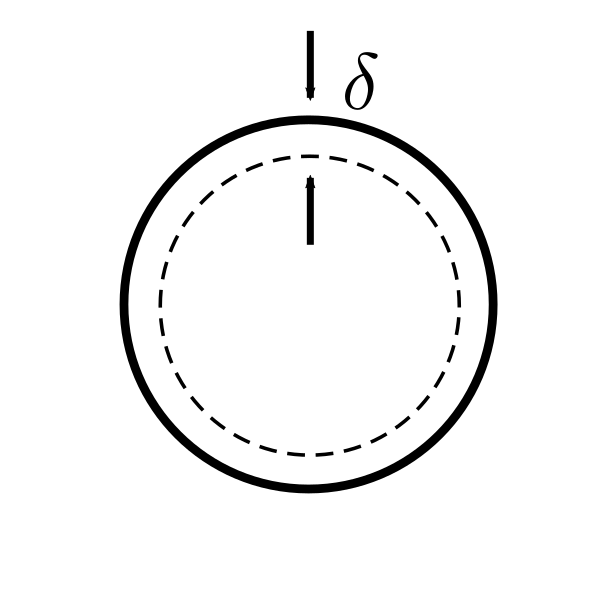
\includegraphics[height=3cm]{error_types/diameter_error_schematic.png}
    \label{fig:diameter_error_schematic}
}
\hspace{5mm}
\subfloat[周方向2山誤差]{
    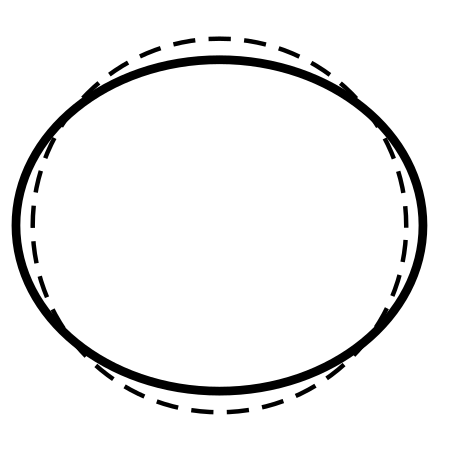
\includegraphics[height=3cm]{error_types/oval_error_schematic.png}
    \label{fig:oval_error_schematic}
}
\hspace{5mm}
\subfloat[周方向中周期誤差]{
    \includegraphics[height=3cm]{error_types/roundness_medium_error_schematic.png}
    \label{fig:roundness_medium_error_schematic}
}
\hspace{5mm}
\subfloat[周方向短周期誤差]{
    \includegraphics[height=3cm]{error_types/roundness_short_error_schematic.png}
    \label{fig:roundness_short_error_schematic}
}
\\

\subfloat[テーパー角誤差]{
    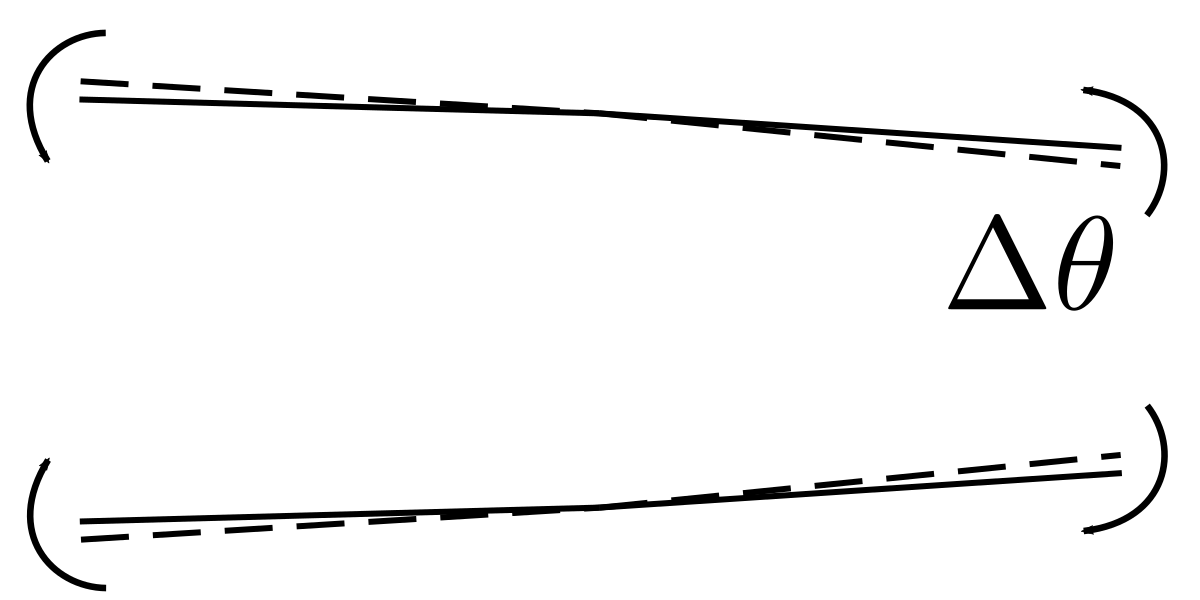
\includegraphics[height=3cm]{error_types/taper_error_schematic.png}
    \label{fig:taper_error_schematic}
}
\hspace{5mm}
\subfloat[光軸たわみ]{
    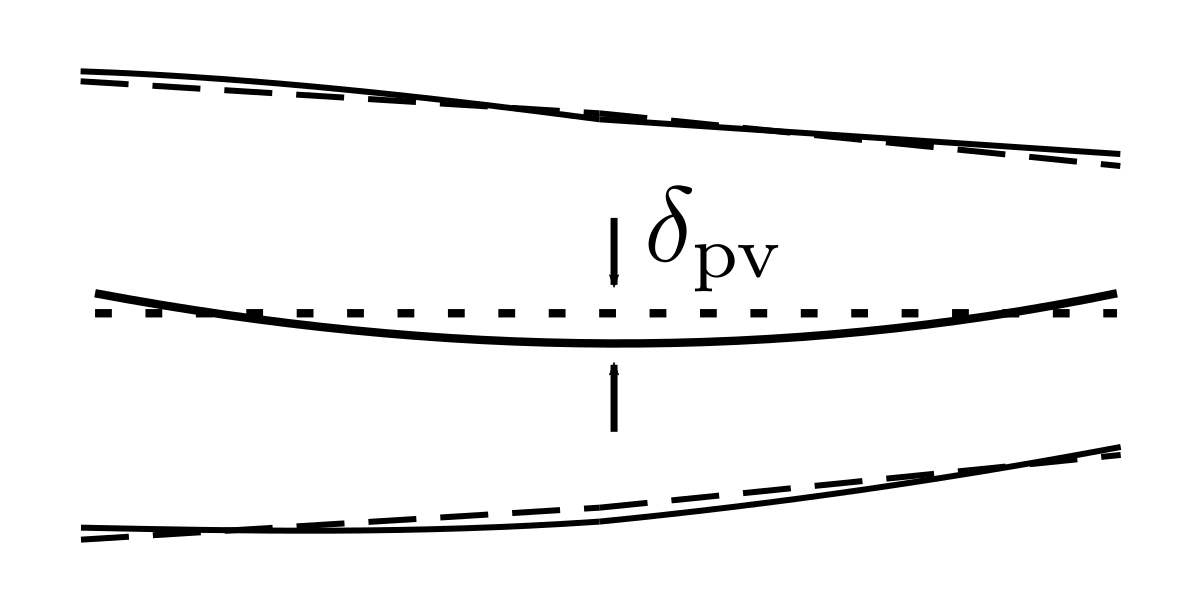
\includegraphics[height=3cm]{error_types/axis_deflection_schematic.png}
    \label{fig:axis_deflection_schematic}
}
\\

\subfloat[長手方向長周期形状誤差]{
    \includegraphics[height=3cm]{error_types/profile_long_error_schematic.png}
    \label{fig:profile_long_error_schematic}
}
\hspace{5mm}
\subfloat[長手方向中周期形状誤差]{
    \includegraphics[height=3cm]{error_types/profile_medium_error_schematic.png}
    \label{fig:profile_medium_error_schematic}
}

\caption[]{入力するミラー形状誤差の種類}
\label{fig:fwhm_explanation}
\end{figure}

\clearpage
% ================================================== %
% section
% ================================================== %
\newpage

\section{理想集光}
\label{chap2_ideal_focusing}

まず、誤差入力を与える前に、誤差のない理想的なミラー形状に対する集光面強度分布を計算し、その特徴について述べる。

\begin{comment}
\begin{figure}[!ht]
\centering

\subfloat[可視光(632.8nm)]{
    \includegraphics[width=3cm]{ideal/visible_light_focus_abs.png}
    \label{fig:visible_light_ideal_focus_abs}
}
\subfloat[4keV]{
    \centering
    \includegraphics[width=3cm]{ideal/3keV_focus_abs.png}
    \label{fig:4keV_ideal_focus_abs}
}
\caption[]{理想的なミラーの各波長に対する集光波面}
\label{fig:fwhm_explanation}
\end{figure}
\end{comment}

表\ref{tb:ideal_focus_evaluation}にそれぞれの波長に対するHPDおよびFWHMを示す。
理想集光の場合は集光波面が回転対象になっているため、FWHMは任意の横方向の1本のプロファイルに対してのみ示す。

\begin{table}[!ht]
\begin{center}
  \begin{tabular}{|c|c|c|} \hline
    項目 & 可視光(632.8nm) & 4keV \\ \hline
    HPD & 8.989 mm & \SI{19.45}{\micro \metre} \\
    FWHM & \SI{19.53}{\micro \metre} & \SI{0}{\micro \metre} \\ \hline
  \end{tabular}
  \caption{理想集光の場合のHPDおよびFWHM}
  \label{tb:ideal_focus_evaluation}
\end{center}
\end{table}

\clearpage
% ================================================== %
% section
% ================================================== %
\newpage

\section{各誤差入力に対するシミュレーション}
\label{chap2_simulation_error_response}

\subsection{X線に対する許容誤差量の解析}
\label{chap2_xray_allowed_error}

まず、4 keV のX線を光源とした場合について、回折限界集光および目標のHPDを達成する上で許容される最大の誤差量を求める。

\begin{table}[!ht]
\begin{center}
  \begin{tabular}{|c|c|c|} \hline
    形状誤差の種類 & Strehl比0.8 & HPD 1 秒角 \\ \hline
    (\ref{sub@fig:diameter_error_schematic}) 直径誤差 & 0.0 mm & 0.0 mm
  \end{tabular}
  \caption{理想集光の場合のHPDおよびFWHM}
  \label{tb:xray_allowed_error}
\end{center}
\end{table}


\clearpage
% ================================================== %
% section
% ================================================== %
\newpage
\section{収差解析}
\label{chap2_simulation_zernike_analysis}

\ref{chap2_simulation_error_response}節では、ミラー加工において生じる様々な誤差を紹介するとともに、その誤差入力についてのシミュレーションを行った。
本節では、\ref{chap3}章で述べる位相回復によって得られた波面情報から各誤差への分解を行うための解析方法について検討する。

\subsection{Zernike収差}

\subsection{輪帯状の位相分布に対するZernike収差}


\subsection{各誤差に起因する収差の解析}



\section{結言}
\label{chap2_conclusion}



%%%%%%%%%%%%%%%%%%%%%%%%%%%%%%%%%%%%%%%%%%%%%%%%%%%%%%%%%%%%%%%%%%%%%%%%%%%%%
%%% Local Variables:
%%% mode: katex
%%% TeX-master: "../thesis"
%%% End:

\chapter{Wolterミラー評価実験の手法に関する検討}
\thispagestyle{empty}
\label{chap3}
\graphicspath{{chap3/figure/}}
\minitoc

\newpage
%%%%%%%%%%%%%%%%%%%%%%%%%%%%%%%%%%%%%%%%%%%%%%%%%%%%%%%%%%%%%%%%%%%%%%%%%%%%%


% ================================================== %
% section
% ================================================== %
\section{諸言}
\label{chap3_introduction}

2章では、Wolterミラーの誤差応答シミュレーションを行い、各種形状誤差によって生じる波面誤差分布を計算した。
本研究の目的であるミラー上の形状誤差量の測定は、それぞれの誤差に対応する波面誤差分布を基底としてミラー下流端面における波面を分解することによってなされる。
本章では、波面計測に用いる位相回復法について基礎的な理論を述べた上で様々な手法について検討し、計測に用いる手法を決定、提案する。
また、提案された手法について測定対象の天文用Wolterミラーに合わせたシミュレーションを行い、その有効性を確認する。

\clearpage
% ================================================== %
% section
% ================================================== %
\newpage

\section{手法の決定に関する方針}
\label{chap3_method_choice_policy}

本節では、手法の検討に先立って、計測方法に対して要請される事項について述べる。

\subsection{高空間分解能}
\label{chap3_high_spatial_resolution}
1章で述べたように、測定対象となるWolterミラーで波面計測を行う際の大きな問題点は、2回反射されたビームが非常に細い輪帯形状をなすことである。
この極めて細い輪帯波面を測定し、形状誤差の情報を計算するためには、形状誤差が波面の動径方向に与える変化を十分な空間分解能で計算できなければならない。
当然、動径方向分解能が高くなるほど長手方向の形状誤差の位置分解能も上がるが、ここでは最低限の条件として3次のコマ収差を検出できること、すなわち動径方向に3画素の分解能を持つことを要請として定める。

\subsection{ダイナミックレンジ}
\label{chap3_dynamic_range}

位相回復計算を行う上で非常に重要な要素の1つが、カメラのダイナミックレンジである。
測定する強度分布において一定値を下回る点では強度が0として検出されてしまうため、同じ強度分布を持つ系であっても回復計算に対して有効な領域はダイナミックレンジによって左右される。
逆に、同じダイナミックレンジに対して有効な領域の大小によって回復計算の収束性や得られる情報の質が変化する。
本研究で用いるCCDカメラのパラメータは表\ref{tb:ccd_camera_params}の通りであり、これに対して回復計算が実行できるような手法であることが要請される。

\begin{table}[!ht]
\begin{center}
  \begin{tabular}{|c|c|l|} \hline
    項目 & 値 \\ \hline
    製品名 & Bitran BQ-85M \\
    ピクセルサイズ & 9.0 um \\
    画素 & 4096 $\times$ 4096 \\
    受光面積 & 36.8 mm $\times$ 36.8 mm \\
    A/Dコンバータ & 16bit (65535階調) \\ \hline
  \end{tabular}
  \caption{CCDカメラのパラメータ}
  \label{tb:ccd_camera_params}
\end{center}
\end{table}

また、実際の撮影時にはノイズが混入するため、ダイナミックレンジはカメラ自体の値より小さくなる。
以下は10回のダークフレーム撮影結果である。


\clearpage
\newpage

% ================================================== %
% section
% ================================================== %

\section{位相回復法の概要}
\label{chap3_phase_retrieval_introduction}

2章でも述べたように、波面計測は波動光学に基づいており、光波は複素スカラー場として表現される。
複素スカラー場の各点において、位相は波面に対応し、絶対値の2乗が強度に対応する。
ゆえに波面計測とは位相分布を求めることに他ならないが、位相を直接測定することは出来ず、CCDなどの受光素子では強度値のみが計測可能である。
つまり、強度分布の計測値から位相分布を算出すること、より具体的には$N \times N$の強度計測値を元に$N \times N$の位相分布を求めることが位相回復法において解かれるべき問題である。
一般にこれは位相回復問題と呼ばれる。
位相回復法には様々な手法が存在するが、いずれの方法においても基本的な方針は共通している。
未知数をすべて決定するためには未知数を含む十分本数の方程式が立式される必要がある。
しかし一般に、求める光学波動場において強度と位相の間に拘束関係はない。
そこで、焦点面に加えてもう1つ平面を定義し、その平面と焦点面の間の光学波動場の伝播を関係式として与えることで、未知数は増えるもののそれらを含む方程式を得ることができる。
これを図\ref{fig:phase_retrieval_policy}に示す。
波動場の伝播はKirhihoff-Helmholtz方程式の解として表され、距離や開口サイズに応じて近似公式が多く知られている。中でも、十分遠方においてフーリエ変換の関係で表されることが知られている。これについては、appendixにおいて詳説する。
波動場の伝播は$n \times n$の離散領域に対して$n \times n$本の数式で表される。
これだけでは未知数が$3n \times n$個に対して方程式が$n \times n$本と少なく、未知数を全て決定することができない。
そこで、未知数を減らす、もしくは関係式を増やすといった工夫を行うことで、解を決定するという方針を取る。

\begin{figure}[!ht]
\centering
\includegraphics[width=11cm]{phase_retrieval_problem.png}
\caption{位相回復問題}
\label{fig:phase_retrieval_problem}
\end{figure}

\begin{figure}[!ht]
\centering
\includegraphics[width=13cm]{phase_retrieval_policy.png}
\caption{位相回復法の方針}
\label{fig:phase_retrieval_policy}
\end{figure}

以下では、代表的な解法を紹介し、続いてそれらを用いた天文用Wolterミラーの波面に対する位相回復法の検討・シミュレーションを行う。


\clearpage
% ================================================== %
% section
% ================================================== %
\newpage

\section{孤立条件の利用}
\label{chap3_solitude_introduction}
主にCDI(コヒーレント回折イメージング)の文脈において、波動場が到達しない領域を定数0として与えることで、未知数をの総数を激減させるという方法が多く取られる。
CDIとは、図\ref{fig:cdi_schematic}に示すように、サンプルに集光ビームを照射し、その回折像を見ることでそのサンプルの内部構造を解析する方法である。

\begin{figure}[!ht]
\centering
\includegraphics[width=12cm]{cdi_schematic.png}
\caption{コヒーレント回折イメージングの概要}
\label{fig:cdi_schematic}
\end{figure}

位相回復法によってディテクターでの位相およびサンプル面における位相・強度を求めることで、サンプル各点における透過率を求めることが目標となる。
このような系においては、カメラの画素をより細かく取ることにより、対応するサンプル面での領域がサンプルより大きく広がるため、この領域には波面が存在しないという仮定を用いて回復計算を行うことができる。
本研究で対象とするWolterミラーについても、回復の対象である輪帯状でかつ細い波面の面積が下流端開口面全体に対して非常に小さく、同様の方法が有効である可能性がある。
この方針に則って、位相回復計算を行う最もシンプルなアルゴリズムがBIO(Basic Input-Output) Algorithmである。
疑似コードをAlgorithm\ref{alg:bio}に示す。

\newcommand{\pos} {
    \mathbf{r}
}
\newcommand{\rpos} {
    \mathbf{q}
}

\begin{algorithm}                      
\caption{BIO Algorithm}         
\label{alg:bio}                          
\begin{algorithmic}
    \STATE $\phi_0(\pos)$
      = $\begin{cases}
        \mathrm{rand} & (\pos \in S) \\
        0 & (\pos \notin S)
      \end{cases}$
    \FOR{n = 0 \ldots N-1}
    \STATE $\Psi_n(\rpos) = \mathcal F [\phi_n(\pos)]$
    \STATE $\Psi_{n+1}(\rpos) = \sqrt{I(\rpos)} \exp \left( i \arg \Psi_n(\rpos) \right)$ 
    \STATE $\phi_n'(\pos) = \mathcal F^{-1} [\Psi_{n+1}(\rpos)]$
    \STATE $\phi_{n+1}(\pos)
      = \begin{cases}
          \phi_n'(\pos) & (\pos \in S) \\
          0 & (\pos \notin S)
      \end{cases}$
    \ENDFOR
\end{algorithmic}
\end{algorithm}

これを改良し、サポートによる射影を弱めることで収束性を高めたのが、HIO(Hybrid Input-Output) Algorithmである。
疑似コードはAlgorithm\ref{alg:hio}のようになる。

\begin{algorithm}                      
\caption{HIO Algorithm}         
\label{alg:hio}                          
\begin{algorithmic}
    \STATE $\phi_0(\pos)$
      = $\begin{cases}
        \mathrm{rand}(0,1) & (\pos \in S) \\
        0 & (\pos \notin S)
      \end{cases}$
    \FOR{n = 0 \ldots N-1}
    \STATE $\Psi_n(\rpos) = \mathcal F [\phi_n(\pos)]$
    \STATE $\Psi_{n+1}(\rpos) = \sqrt{I(\rpos)} \exp \left( i \arg \Psi_n(\rpos) \right)$ 
    \STATE $\phi_n'(\pos) = \mathcal F^{-1} [\Psi_{n+1}(\rpos)]$
    \STATE $\phi_{n+1}(\pos)
      = \begin{cases}
          \phi_n'(\pos) & (\pos \in S) \\
          \phi_n(\pos) - \beta \phi_n'(\pos) & (\pos \notin S)
      \end{cases}$
    \ENDFOR
\end{algorithmic}
\end{algorithm}

位相回復計算が収束するかどうかを決める最大の要因の1つが、オーバーサンプリング比、つまり試料に対してどれだけ大きな領域を取って計算できるかということである。
これは、カメラの空間分解能によって決まる。
位相回復計算が収束するために必要な最低限の条件として、FFTで結ばれる関係式の数が未知数の数を上回らなければならない。
Friedel則による対称性などを考慮すると、取得する総ピクセル数が回復する試料のピクセル数の2倍になっていなければいけないことになる。\cite{Latychevskaia2018}
実際にはノイズが乗ったり、直接通過する光が入射しないようにビームストップを配置したりといった事情から、2倍より大きくなければならない。

\clearpage
% ================================================== %
% section
% ================================================== %
\newpage

\section{タイコグラフィ法}
\label{chap3_ptychography_introduction}
\subsection{タイコグラフィ法の概要}
\ref{chap3_solitude_introduction}節では1枚の画像に対して孤立条件から冗長性を確保して位相回復を行ったが、タイコグラフィ法では光学系に徐々に変化を与えながら、多数の画像を撮影することによって冗長性を確保する。
図\ref{fig:ptychography_schematic}にその概要を示す。

\begin{figure}[!ht]
\centering
\includegraphics[width=12cm]{ptychography_schematic.png}
\caption{タイコグラフィ法の概要}
\label{fig:ptychography_schematic}
\end{figure}

集光ミラーに設計時に想定された光源からの入射光を入れ、その焦点面にオブジェクトを差し入れる。
このオブジェクトによって変化を受けた波面がさらに下流側に設置されたカメラによって撮影される。
これを、オブジェクトの位置を焦点面内で鉛直および水平方向に走査しながら多数の画像を撮影することで、冗長性を確保するという寸法である。
用いるオブジェクトは大きく分けて2種類ある。
1つはガラスなどの透過性を持つ物体の厚みに適当なパターンを与えた試料をオブジェクトとするものである。
物体の厚みを位置によって変えることで、それに応じて波面の位相の進み量に差が生じる。
試料の作製については、SiO2のエッチングによるパターニングなどが知られている。\cite{Godden2016}
この方法は、タイコグラフィによるミラー評価だけでなく、試料そのものを評価するタイコグラフィ顕微鏡としても利用できる。
もう1つは、ビームを完全に遮蔽できるような金属板に適当な穴を開けて作られるオブジェクトである。
焦点面における波面は完全に遮蔽される部分と完全に透過される部分の2つに分かれ、透過した波面の穴のエッジで回折した光が下流側のカメラに入射する。
これらのオブジェクトを焦点面内で走査し、各位置に対する回折光を

竹尾らは、ピンホール(1つの円形の穴)を開けた板をオブジェクトとして利用し、ピンホールのエッジをなぞるように走査する方法でタイコグラフィを行い、ミラー内面形状の評価に成功している。
ピンホールを用いた方法では、ミラーの内側で反射せず直接通過した光を処理することが位相パターンをつけた試料より容易である。

\subsection{PIE}
位相回復法は元来、X線顕微鏡として利用されたため、回復の対象はサンプル(オブジェクト)であった。
その最も簡単なタイコグラフィのアルゴリズムがPIE(Ptychography Iterative Engine)である。
これは、照明関数は既知であるとして与え、オブジェクトのみ回復計算を行うアルゴリズムである。
PIEの疑似コードをAlgorighm\ref{alg:pie}に示す。

\begin{algorithm}                      
\caption{PIE Algorithm}         
\label{alg:pie}                          
\begin{algorithmic}
    \STATE $O_0(\pos) = \mathrm{rand}(0,1) \exp(i \mathrm{rand}(0,1) )$
    \FOR{n = 0 \ldots N-1}
      \FOR{j = 0 \ldots M-1}
        \STATE $\psi(\pos_j) = P(\pos) O_n(\pos_j + \pos)$
        \STATE $\Psi(\rpos) = \mathcal F [\psi(\pos)]$
        \STATE $\Psi'(\rpos) = \sqrt{I_j(\rpos)} \exp\left( i \arg \psi(\pos) \right)$ 
        \STATE $\psi'(\pos) = \mathcal F^{-1} [\Psi'(\rpos)]$
        \STATE $O_{n+1}(\pos + \pos_j)'
          = O_n(\pos + \pos_j) 
          + \frac{P_n^*(\pos)}{|P(\pos)|^2+\varepsilon} \left( \psi_n'(\pos) - \psi_n(\pos) \right)$
      \ENDFOR
    \ENDFOR
\end{algorithmic}
\end{algorithm}

逆空間で拘束を掛け、実空間に戻したあとで、オブジェクトを更新する。
オブジェクトの更新則としてシンプルなのは$\psi(\pos_j) = P(\pos) O_n(\pos_j + \pos)$としたのに対応させて$O_{n+1}(\pos_j + \pos) = \frac{\psi'(\pos_j)}{P(\pos)}$とする方法である。
しかし、これは除算に際して発散が起こる可能性があり、実用上大きな問題を孕んでいる。
これを、式\ref{eqn:object_update_derivation}のように変形する。
\begin{eqnarray}
O_{n+1}(\pos_j + \pos)
  &=& \frac{\psi'(\pos_j)}{P(\pos)} \nonumber \\
  &=& \left( O_n(\pos_j + \pos) - \frac{\psi(\pos_j)}{P(\pos)} \right) + \frac{\psi'(\pos_j)}{P_n(\pos)} \nonumber \\
  &=& O_n(\pos_j + \pos) + \frac{1}{P(\pos)} \left( \psi'(\pos_j) - \psi(\pos_j) \right) \label{eqn:object_update_derivation}
\end{eqnarray}

これを一般化して文字を置き換えると、式\ref{eqn:object_update_simplified}のように書ける。
\begin{equation}
\label{eqn:object_update_simplified}
  O_{n+1}(\pos_j + \pos) = O_n(\pos_j + \pos) + w \Delta\psi(\pos)
\end{equation}
この更新の重み$w$を変えることで、アルゴリズムの改善を図る。
発散を回避するため、重みの分母を実数化して微小な定数$\varepsilon$を足して式\ref{eqn:pie_object_update_weight}のように重みを定めたのがAlgorithm\ref{alg:pie}に示したPIEのアルゴリズムである。
\begin{equation}
  \label{eqn:pie_object_update_weight}
  w = \frac{P*(\pos)}{\left| P(\pos) \right|^2 + \varepsilon}
\end{equation}

\subsection{rPIE}
PIEがオブジェクトのみ回復を行っていたのに対して、照明関数も未知として回復計算を行うのがePIE(exteded PIE)である。
ePIEでは式\ref{eqn:pie_object_update_weight}のように定数で発散を回避するのではなく、式\ref{eqn:epie_object_update_weight}のように絶対値の2乗の最大値を取る。
また、更新係数にハイパーパラメタ$\alpha$を掛けることで収束性を上げることができることが知られている。
\begin{equation}
  \label{eqn:epie_object_update_weight}
  w = \alpha \frac{P_n*(\pos)}{\max \left| P_n(\pos) \right|^2}
\end{equation}
ePIEでは照明関数も更新しなければいけないが、これはオブジェクトの更新と同様に式\ref{eqn:epie_probe_update}のように行われる。
\begin{equation}
\label{eqn:epie_probe_update}
  P_{n+1}(\pos) 
  = P_n(\pos) 
  + \beta \frac{O_n*(\pos_j + \pos)}{\max \left| O_n(\pos_j + \pos) \right|^2} \Delta\psi(\pos)
\end{equation}

ePIE(式\ref{eqn:epie_object_update_weight})のように最大値を取る方法に対して、各点での絶対値の2乗とその最大値で重み付き平均を取って分母とするのがrPIE(regularized PIE)である。
更新式は式\ref{eqn:rpie_object_update}および式\ref{eqn:rpie_probe_update}に示す通りである。
rPIEはほとんどePIEの一般化になっている。
\begin{eqnarray}
  O_{n+1}(\pos_j + \pos) &=& O_n(\pos_j + \pos) 
    + \frac{P_n*(\pos_j + \pos)}
      {\alpha \max \left| P_n(\pos) \right|^2 + (1-\alpha) \left| P_n(\pos) \right|^2}
    \Delta\psi(\pos) \label{eqn:rpie_object_update} \\
  P_{n+1}(\pos) &=& P_n(\pos) 
    + \frac{O_n*(\pos_j + \pos)}
      {\beta \max \left| O_n(\pos_j + \pos) \right|^2 + (1-\beta) \left| O_n(\pos_j + \pos) \right|^2}
    \Delta\psi(\pos) \label{eqn:rpie_probe_update}
\end{eqnarray}

rPIEのアルゴリズムをAlgorithm\ref{alg:rpie}に示す。

\begin{algorithm}                      
\caption{rPIE Algorithm}         
\label{alg:rpie}                          
\begin{algorithmic}
    \STATE $O_0(\pos) = \mathrm{rand}(0,1) \exp(i \mathrm{rand}(0,1) )$
    \STATE $P_0(\pos) = \mathrm{rand}(0,1) \exp(i \mathrm{rand}(0,1) )$
    \FOR{n = 0 \ldots N-1}
      \FOR{j = 0 \ldots M-1}
        \STATE $\psi(\pos_j) = P_n(\pos) O(\pos_j + \pos)$
        \STATE $\Psi(\rpos) = \mathcal F [\psi(\pos)]$
        \STATE $\Psi'(\rpos) = \sqrt{I_j(\rpos)} \exp\left( i \arg \psi(\pos) \right)$ 
        \STATE $\psi'(\pos) = \mathcal F^{-1} [\Psi'(\rpos)]$
        \STATE $O_{n+1}(\pos_j + \pos) 
          = O_n(\pos_j + \pos) + \frac{P_n*(\pos_j + \pos)}
          {\alpha \max \left| P_n(\pos) \right|^2 + (1-\alpha) \left| P_n(\pos) \right|^2}
          \Delta\psi(\pos)$
        \STATE $P_{n+1}(\pos)
          = P_n(\pos) + \frac{O_n*(\pos_j + \pos)}
          {\beta \max \left| O_n(\pos_j + \pos) \right|^2 + (1-\beta) \left| O_n(\pos_j + \pos) \right|^2}
          \Delta\psi(\pos)$
      \ENDFOR
    \ENDFOR
\end{algorithmic}
\end{algorithm}

タイコグラフィ法においても、走査ステップを変えることで回復領域の重なり具合が変化し、この比(オーバーサンプリング比)が収束性を左右する。
ステップが小さいほどオーバーサンプリング比は大きく収束性は高くなるが、その分必要な領域を走査し終えるのに必要な計測時間は増大してしまう。
Bunkらの検討によれば、オーバーサンプリング比が0.6程度が最適であるということが知られている。\cite{Bunk2008}

\subsection{Wolterミラー計測への適用}
Wolterミラー計測
ピンホールをオブジェクトとして用いるタイコグラフィ法でシミュレーションを行う。

\clearpage
% ================================================== %
% section
% ================================================== %
\newpage

\section{ディテクター走査による冗長性}

タイコグラフィ法ではオブジェクトを走査することで冗長性を確保したが、ディテクターを走査することで冗長性を確保する方法も知られている。

\begin{figure}[!ht]
\centering
\includegraphics[width=12cm]{detector_scanning_schematic.png}
\caption{ディテクターを走査する方法の概要}
\label{fig:detector_scanning_schematic}
\end{figure}


\clearpage
% ================================================== %
% section
% ================================================== %
\newpage

\section{下流端開口走査による冗長性}

オブジェクトを走査する位置を焦点面ではなく集光素子の開口直後とするTransverse Translation法がBradyらによって提案されている。\cite{Brady2009}
これは図\ref{fig:transverse_schematic}に示すように、焦点面を操作するタイコグラフィ法同様にオブジェクトを集光素子の開口で走査し、その回折像を下流側のカメラで撮影するという方法である。

\begin{figure}[!ht]
\centering
\includegraphics[width=12cm]{transverse_schematic.png}
\caption{Transverse Translation Diversityの概要}
\label{fig:transverse_schematic}
\end{figure}

計算アルゴリズム自体は基本的にはタイコグラフィ法と同様にすればよい。
タイコグラフィ法と構成が異なるため、同じ装置・素子に対して計算条件や分解能が異なる。

\subsection{対称性}

\clearpage
% ================================================== %
% section
% ================================================== %
\newpage


\section{結論}
\label{chap3_conclusion}
結論を述べる。




%%%%%%%%%%%%%%%%%%%%%%%%%%%%%%%%%%%%%%%%%%%%%%%%%%%%%%%%%%%%%%%%%%%%%%%%%%%%%
%%% Local Variables:
%%% mode: katex
%%% TeX-master: "../thesis"
%%% End:

%\chapter{レンズによる提案手法の検討}
\thispagestyle{empty}
\label{chap4}
\graphicspath{{chap4/figure/}}
\minitoc

\newpage
%%%%%%%%%%%%%%%%%%%%%%%%%%%%%%%%%%%%%%%%%%%%%%%%%%%%%%%%%%%%%%%%%%%%%%%%%%%%%


% ================================================== %
% section
% ================================================== %
\section{諸言}
\label{chap4_introduction}

本章では5章のミラー測定実験に先立って、ほぼ理想的と言える集光光学系に対して3章で提案された手法による計測実験を行い、その正当性を検証する。
具体的な方法としては、平行光に対して輪帯状の開口を入れ、さらにレンズによって集光することで、輪帯状の集光球面波を作ることができ、擬似的にミラー下流端面を再現する。
再現された擬似的な輪帯に対して位相回復法が適用出来れば、細い輪帯形状の波面回復法に対して提案手法が有効的であることがいえ、また本研究の測定対象である天文用Wolterミラーに対してもその適用可能性が大きいということが言える。
また、1層のWolterミラーの波面計測のための手法検討に加えて、Nested Wolterミラーにも同手法が適用可能であるかどうかを検討するための実験を行う。
現時点では入手性の観点から実際のNested Wolterミラーを計測することは難しいが、Nested Wolterミラーの集光波面を模倣した輪帯に対して位相回復法が機能すれば、十分に応用可能であることの根拠を与える。
\ref{chap4_experiment_setup}節では、実験の構成およびそれに含まれる各光学素子のパラメータ等について示す。


\clearpage
% ================================================== %
% section
% ================================================== %
\newpage

\section{実験の構成および設計パラメータ}
\label{chap4_experiment_setup}

\ref{chap4_introduction}節で述べたとおり、本章ではほぼ理想的な輪帯上の集光波面を擬似的に生成し、これに対して波面計測を行う。
輪帯上の集光波面は、図\ref{fig:psuedo_focusing_ring_model}に示すように輪帯アパーチャ及び集光レンズによって生成される。

\begin{figure}[!ht]
\centering
\includegraphics[width=13cm]{psuedo_focusing_ring.png}
\caption{疑似的な輪帯状集光ビームの生成}
\label{fig:psuedo_focusing_ring_model}
\end{figure}

疑似輪帯を用いた計測実験は、本来の測定対象であるWolterミラーと同様の光学的パラメータで構成されるべきだが、入手性の問題からここではレンズとして口径は異なるがNAがWolterミラーのそれとほぼ等しいレンズを用いる。
用いたレンズのパラメータは表\ref{tb:focusing_lens_params}に示す通りである。

\begin{table}[h]
\begin{center}
  \begin{tabular}{|c|c|} \hline
    パラメータ & 値 \\ \hline
    直径 & 30.0 mm  \\
    焦点距離 & 1000.000 mm \\
    設計波長 & 541.6 nm \\ \hline
  \end{tabular}
  \caption{レンズの設計パラメータ}
  \label{tb:focusing_lens_params}
\end{center}
\end{table}

これに合わせて、輪帯開口および位相回復に用いるピンホールを図\ref{fig:lens_pinhole_ring_aperture}の用に設計した。

\begin{figure}[!ht]
\centering

\subfloat[輪帯アパーチャ]{
    \centering
    \includegraphics[width=6cm]{ring_aperture.png}
    \label{fig:lens_ring_aperture}
}
\subfloat[ピンホール]{
    \centering
    \includegraphics[width=6cm]{pinhole_arrangement.png}
    \label{fig:lens_pinhole_arrangement}
}
\caption[]{設計図面}
\label{fig:lens_pinhole_ring_aperture}
\end{figure}

\clearpage
% ================================================== %
% section
% ================================================== %
\newpage


\section{疎条件を利用した位相回復の結果}
回復計算に用いたパラメータは以下の通りである。

回復計算が収束しなかった。


\clearpage
% ================================================== %
% section
% ================================================== %
\newpage

\section{下流端走査によるタイコグラフィの結果}


\subsection{半周のみ走査した場合のタイコグラフィの結果}

\subsection{繰り返し計測の結果}

像が回復できることが確認されたため、さらに10回の繰り返し計測を行い、繰り返し再現性およびその波面計測の精度を確認する。


\clearpage
% ================================================== %
% section
% ================================================== %
\newpage

\section{Nested Wolterミラーに対する下流端走査型位相回復法の検証}

1層の場合と同様に、輪帯状の集光波面が同心円状に2つ存在するような状況を擬似的に作り出し、これを計測する。
アパーチャとピンホールの設計を図\ref{fig:lens_nested_pinhole_ring_aperture}に示す。

\begin{figure}[!ht]
\centering

\subfloat[輪帯アパーチャ]{
    \centering
    \includegraphics[width=6cm]{nested_ring_aperture.png}
    \label{fig:lens_nested_ring_aperture}
}
\subfloat[ピンホール]{
    \centering
    \includegraphics[width=6cm]{nested_pinhole_arrangement.png}
    \label{fig:lens_nested_pinhole_arrangement}
}
\caption[]{疑似Nested Wolter計測用の設計図面}
\label{fig:lens_nested_pinhole_ring_aperture}
\end{figure}

\subsection{結果}

回復された波面の強度分布を図\ref{fig:result_nested_restored_abs}に示す。

\begin{figure}[!ht]
\centering
\includegraphics[width=6cm]{result_nested/restored_abs.png}
\caption{疑似的な輪帯状集光ビームの生成}
\label{fig:result_nested_restroed_abs}
\end{figure}



\clearpage
% ================================================== %
% section
% ================================================== %
\newpage


\section{結論}
\label{chap4_conclusion}


%%%%%%%%%%%%%%%%%%%%%%%%%%%%%%%%%%%%%%%%%%%%%%%%%%%%%%%%%%%%%%%%%%%%%%%%%%%%%
%%% Local Variables:
%%% mode: katex
%%% TeX-master: "../thesis"
%%% End:

\chapter{ミラー計測実験}
\thispagestyle{empty}
\label{chap5}
\graphicspath{{chap5/figure/}}
\minitoc

\newpage
%%%%%%%%%%%%%%%%%%%%%%%%%%%%%%%%%%%%%%%%%%%%%%%%%%%%%%%%%%%%%%%%%%%%%%%%%%%%%


% ================================================== %
% section
% ================================================== %
\section{諸言}
\label{chap5_introduction}

本章では、実際に天文用Wolterミラーを\ref{chap3}章の提案手法による計測実験を行い、その解析を行う。
測定対象となるミラーは、2019年2月および同年9月に作製されたWolterミラーであり、それぞれについて位相回復計算を行った結果およびそこから計算される形状誤差について述べる。
また、これらは既に〇〇によって真円度測定がなされており、計測結果と真円度測定結果との比較・検討を行う。

\clearpage
% ================================================== %
% section
% ================================================== %
\newpage

\section{実験の構成}

実験装置の概要を図\ref{fig:mirror_experiment_schematic}に示す。
まず、レーザーからビームを出力し、これをNDフィルタによって減衰させ、強度を調整する。
次に、レンズを2つ使ってビームを拡大し平行化する。
これを測定対象のWolterミラーに入射し、さらにタイコグラフィのための回転ピンホールを通過させる。
最後に、一番下流にあるCCDカメラで強度分布を撮影する。

\begin{figure}[!ht]
\centering
\includegraphics[width=14cm]{schematic.png}
\caption{ミラー測定実験系 模式図}
\label{fig:mirror_experiment_schematic}
\end{figure}

これらの光学素子のパラメータを表\ref{}に示す。
なお、NDフィルタは実験によって適宜ピークがダイナミックレンジに収まるように設定されるため、そのパラメータ等を記述しない。

\begin{table}[h]
\begin{center}
  \begin{tabular}{|c|c|} \hline
    パラメータ & 値 \\ \hline
    拡大用レンズ & 30.0 mm  \\
    拡大倍率 & 100 倍 \\
    設計波長 & 541.6 nm \\ \hline
  \end{tabular}
  \caption{Wolterミラー計測実験装置における各素子のパラメータ}
  \label{tb:mirror_experiment_params}
\end{center}
\end{table}


これらを構成した実験装置のCAD図を以下に示す。図\ref{fig:mirror_experiment_asm_cad_side}が横から見た図、図\ref{fig:mirror_experiment_asm_cad_isometric}が俯瞰して見た図である。

\begin{figure}[!ht]
\centering
\includegraphics[width=14cm]{setup/asm_total_side.png}
\caption{ミラー測定実験系 側面図}
\label{fig:mirror_experiment_asm_cad_side}
\end{figure}

\begin{figure}[!ht]
\centering
\includegraphics[width=10cm]{setup/asm_total_isometric.png}
\caption{ミラー測定実験系 俯瞰図}
\label{fig:mirror_experiment_asm_cad_isometric}
\end{figure}

\clearpage

% ================================================== %
% section
% ================================================== %
\newpage

\section{計測波面以外の通過光の処理方法に関する検討}
測定対象となっている天文用Wolterミラーは、X線集光用に設計・作製されたものであり、可視光を入射した際にどのような集光波面が生じるかは未検討である。
特に、可視光はX線に比べ2桁程度波長が長く、回折の影響が顕著であることが大きな差異として存在する。
\ref{chap4}章での提案手法の検討は、あくまで波面計測の対象である輪帯のみが存在する場合について行われたが、実際にミラーを計測する実験においては測定対象以外の光も通過してCCDカメラの方向に進行する。
円盤状に広がる平行光を入射した際にミラーより下流に通過する光は、図\ref{fig:mirror_beam_path_types}に示す通り4種類存在する。

図\ref{fig:mirror_beam_path_types}(a)が、測定対象となる波面、つまり正しく放物面、双曲面の順に2回反射した光である。
これに対して、図\ref{fig:mirror_beam_path_types}(b)の直接通過してCCDカメラに到達する光、
図\ref{fig:mirror_beam_path_types}(c)の放物面に当たらず直接双曲面で反射された光、
図\ref{fig:mirror_beam_path_types}(d)の開口端のエッジで回折して進行する光が存在する。

\begin{figure}[!ht]
\centering
\includegraphics[width=10cm]{setup/asm_total_isometric.png}
\caption{ミラーに入射した光の進路}
\label{fig:mirror_beam_path_types}
\end{figure}

直接通過光は、
\subsection{直接通過光}


\subsection{双曲面で1回反射した光}


\subsection{上流端エッジでの回折光}
\label{chap5_}

\clearpage

% ================================================== %
% section
% ================================================== %
\newpage

\section{可視光ビームによるWolterミラー集光波面強度分布の測定}



\clearpage

% ================================================== %
% section
% ================================================== %
\newpage

\section{下流端走査タイコグラフィの結果}

\clearpage
% ================================================== %
% section
% ================================================== %
\newpage

\section{回復波面の解析}
\subsection{周方向誤差の真円度測定結果との比較}

% ================================================== %
% section
% ================================================== %
\section{結論}
\label{chap5_conclusion}


%%%%%%%%%%%%%%%%%%%%%%%%%%%%%%%%%%%%%%%%%%%%%%%%%%%%%%%%%%%%%%%%%%%%%%%%%%%%%

%%% Local Variables:
%%% mode: katex
%%% TeX-master: "../thesis"
%%% End:

\chapter{結論}
\thispagestyle{empty}
\label{chap6}
\graphicspath{{chap6/figure/}}
\minitoc

\newpage
%%%%%%%%%%%%%%%%%%%%%%%%%%%%%%%%%%%%%%%%%%%%%%%%%%%%%%%%%%%%%%%%%%%%%%%%%%%%%


% ================================================== %
% section
% ================================================== %
\section{提案手法の適用可能性}
\label{chap6_conclusion}




\clearpage


% ================================================== %
% section
% ================================================== %
\newpage

\section{今後の展望}
\label{chap6_futureworks}


\clearpage
\newpage


%%%%%%%%%%%%%%%%%%%%%%%%%%%%%%%%%%%%%%%%%%%%%%%%%%%%%%%%%%%%%%%%%%%%%%%%%%%%%
%%% Local Variables:
%%% mode: katex
%%% TeX-master: "../thesis"
%%% End:


% ++++++++++++++++++++++++++++++++++++++++++++++++++++++++++++++++ %
%   Appendix
% ++++++++++++++++++++++++++++++++++++++++++++++++++++++++++++++++ %
%\appendix
%\chapter{付録}
\lhead[付録]{}
\label{appendix}
\graphicspath{{figure/}}
\minitoc

\newpage
\section{光学波動場の伝播}
\subsection{Kirhihoff-Helmholtz方程式}

\subsection{Rayleigh-Sommerfeldの回折積分公式}

\subsection{Rayleigh-Sommerfeldの高速計算}

\subsection{Fresnel回折積分}

\subsection{Fraunhofer回折積分}

\subsection{角スペクトル法}


%%%%%%%%%%%%%%%%%%%%%%%%%%%%%%%%%%%%%%%%%%%%%%%%%%%%%%%%%%%%%%%%%%%%%%%%%%%%%%%
%%% Local Variables:
%%% mode: katex
%%% TeX-master: "../thesis"
%%% End:

%\cleardoublepage

% ++++++++++++++++++++++++++++++++++++++++++++++++++++++++++++++++ %
%   References
% ++++++++++++++++++++++++++++++++++++++++++++++++++++++++++++++++ %
%\chapter*{参考文献}
%\addcontentsline{toc}{chapter}{参考文献}
%\lhead[参考文献]{}
%\renewcommand{\refname}{引用文献}
\thispagestyle{empty}

\bibliography{references}
\bibliographystyle{junsrt}

\newpage

% ++++++++++++++++++++++++++++++++++++++++++++++++++++++++++++++++ %
%  Acknowledgements
% ++++++++++++++++++++++++++++++++++++++++++++++++++++++++++++++++ %
\chapter*{謝辞}
\if0
\markboth{謝辞}{}
\label{thankyou}
\fi

\lhead[謝辞]{}
\thispagestyle{empty}

\newpage

\if0
感謝


\begin{flushright}
2021年2月 渡辺 貴史
\end{flushright}
\fi
%%%%%%%%%%%%%%%%%%%%%%%%%%%%%%%%%%%%%%%%%%%%%%%%%%%%%%%%%%%%%%%%%%%%%%%%%%%%%%%

%%%%%%%%%%%%%%%%%%%%%%%%%%%%%%%%%%%%%%%%%%%%%%%%%%%%%%%%%%%%%%%%%%%%%%%%%%%%%%%
%%% Local Variables:
%%% mode: katex
%%% TeX-master: "../thesis"
%%% End:

% \addcontentsline{toc}{chapter}{謝辞} %   /* add acknowledgement to the table of contents */

% End of Document
\end{document}